\documentclass[11pt]{article}

\usepackage[utf8]{inputenc}
\usepackage[T1]{fontenc}
\usepackage{charter}
\usepackage{amsmath,amssymb}
\usepackage{booktabs}
\usepackage{graphicx}
\usepackage{xcolor}
\usepackage{microtype}
\usepackage{setspace}
\usepackage{lineno}
\usepackage[hidelinks]{hyperref}
\usepackage[a4paper,margin=2.5cm]{geometry}
\usepackage[font=small,labelfont=bf]{caption}

\doublespacing
\linenumbers
\renewcommand{\arraystretch}{1.15}

\title{Spectral concentration in Vina docking-score matrices: what two-way centering reveals and does not correct}

\author{
Adeliya Leleytner$^{1,*}$, Victor Safronov$^{1}$, Maxim Fedorov$^{1}$\\[4pt]
\small $^{1}$Institute for Information Transmission Problems of the Russian Academy of Sciences\\
\small (Kharkevich Institute), Bolshoy Karetny per. 19, Moscow 127051, Russia\\
\small $^{*}$Correspondence: \texttt{a.leleytner@gmail.com}
}
\date{}

\begin{document}
\maketitle

\begin{abstract}
Reverse docking, off-target profiling and multiobjective design use docking scores as a
ligand-by-target matrix, yet the statistical structure of this matrix can confound shared
score tendencies with target-resolved information. We measured spectral concentration in
two large AutoDock Vina matrices using the participation-ratio (PR) effective dimension of
the target-correlation spectrum. A 12,651-compound by 44-target panel had PR dimension 1.83,
and DOCKSTRING, with 260,060 complete molecules by 58 targets, had PR dimension 2.27.
Removing ligand and target main effects changed the estimand and increased these values to
9.30 and 18.21; paired chemical-cluster resampling placed the increase at 6.98--7.91 in the
44-target panel, and five independent DOCKSTRING chemical supports gave increases of
15.88--16.05. The residual surfaces nevertheless remained concentrated relative to fitted
additive-noise nulls, whose median PR dimensions were 42.40 and 56.48. On a matched
74-compound by six-target ChEMBL surface, the experimental-minus-docking PR difference was
2.01 (paired ligand-bootstrap interval 1.17--2.67) before centering but 0.48
($-0.07$--0.92) afterward. A leave-one-ligand-out target-preference benchmark then separated
spectral structure from operational utility. Absolute Vina scores reached mean pairwise
accuracy 0.619, but a target-offset-only baseline reached 0.625 and ligand-identity
permutation reproduced the absolute-score result ($p=0.638$). Column-standardized and
two-way-residual scores reached 0.537 and 0.540; their paired difference was 0.004
($-0.019$--0.026 by scaffold bootstrap). Two-way centering is therefore useful for
diagnosing residual score structure, but higher residual dimension is not by itself a
validated correction for target ranking.

\medskip\noindent\textbf{Scientific Contribution.} We provide a preprocessing-matched
spectral analysis of two large dense Vina panels and separate uncertainty in chemical and
target-panel composition from transformation effects. A matched experimental benchmark
shows both what two-way centering reveals---higher-dimensional residual structure---and what
it does not establish: improved target ranking.
\end{abstract}

\noindent\textbf{Keywords:} molecular docking; AutoDock Vina; effective dimension; spectral
analysis; two-way centering; reverse docking; target profiling.

\section{Introduction}

A docking score is scalar for one protein--ligand pose, but many applications produce a
matrix. Reverse docking ranks targets for a ligand, secondary-pharmacology panels compare
off-target liabilities, and multiobjective design uses scores against several desired and
undesired proteins. In each case the useful object is a matrix $X\in\mathbb{R}^{N\times P}$
whose rows are ligands and columns are targets. Interpreting its $P$ columns as $P$
independent target-resolved descriptors assumes that the matrix actually contains a
commensurate number of independent directions.

Two long-recognized biases make this assumption doubtful. Empirical energy functions often
reward larger ligands because additional atoms contribute additional favorable contacts;
normalization by molecular weight, heavy-atom count or learned physicochemical corrections
can change virtual-screening rankings.\cite{pan2003,jacobsson2006,carta2007} Across proteins,
scores also depend on pocket contact area, size and hydrophobicity. In a reverse-docking
study of 5,000 molecules and 100 proteins, these target properties produced recurrent
``interference proteins'' and motivated per-target normalization.\cite{luo2017} These
observations identify ligand and target main effects. They do not say how much of a complete
score matrix those effects occupy, how many collective directions remain, or whether a
low-dimensional column-standardized surface is equivalent to poor selectivity.

Two-directional normalization and principal-component analysis of docking matrices also
precede this study. SePreSA applied a ligand-wise Z transformation followed by normalization
of protein-score vectors to a 79-compound by 86-protein docking matrix.
\cite{sepresa2009} Fukunishi and colleagues applied PCA to a complete docking matrix for
compound and pocket classification, and later used multi-protein docking-score profiles as
QSAR descriptors.\cite{fukunishi2006,fukunishi2018} These studies establish that matrix-wide normalization and
PCA are useful. The contribution here is narrower: a large-scale quantitative estimate of
spectral concentration, explicit comparison of column-standardized and two-way-centered
estimands, and uncertainty analyses for chemical and target-panel composition.

The distinction matters because docking has several separable tasks. A method may reproduce
a crystallographic pose yet rank affinities poorly, and no single program performs uniformly
across targets and evaluation objectives.\cite{warren2006} Likewise, the aggregate variance of a
score matrix and the correctness of within-ligand target contrasts are different objects.
Writing
\begin{equation}
X_{ij}=\mu+a_i+b_j+\gamma_{ij},
\label{eq:decomposition}
\end{equation}
separates the grand mean $\mu$, the ligand tendency $a_i$ to score well across targets, the
target tendency $b_j$ to score ligands favorably, and the interaction $\gamma_{ij}$. The
column-standardized spectrum is allowed to be dominated by $a_i$. Selectivity, however, depends on
differences within rows and ultimately on $\gamma_{ij}$; the additive terms cancel from a
double difference. A PR estimate on $X$ and the same estimate on $\gamma$ therefore answer
different questions. Established panel selectivity summaries such as Gini, entropy and
window scores also answer different questions and can reorder the same compounds, making the
metric definition part of the estimand rather than a cosmetic choice.\cite{graczyk2007,bosc2017}

Complete public score matrices now permit this distinction to be tested at useful scale.
DOCKSTRING contains docking scores for more than 260,000 molecules against 58 medically
relevant targets.\cite{dockstring2022} An independent acute-toxicity resource contains
12,651 analyzable compounds docked against a 44-protein secondary-pharmacology
panel.\cite{nikitin2025} We combine these matrices with matched experimental affinity data.
Two small RF-Score rescoring blocks and learned-affinity examples are retained as
illustrative sensitivities in the Supplement because neither provides a large independent
replication of the principal Vina result.\cite{rfscore2010}

Low-rank representations are not new to chemogenomics. Kernelized Bayesian matrix
factorization, probabilistic matrix factorization and neighborhood-regularized latent-factor
models deliberately embed sparse DTI observations in lower-dimensional spaces to improve
prediction or matrix completion.\cite{gonen2012,cobanoglu2013,liu2016} Our question is
different: we do not impose a low-rank predictive model on sparse experimental data. We
measure the empirical spectrum of dense docking output, then ask which part is attributable
to additive ligand and target effects. The two-way decomposition connects this diagnostic to
classical additive-model reasoning, while participation and entropy ranks provide continuous
summaries rather than a chosen latent dimension.\cite{lee2016,roy2007}

We ask four linked questions. Do the two large tested Vina panels concentrate their variance
into a few PR effective dimensions? Is that observation stable to chemical and target-panel
composition? What remains after ligand and target main effects are removed? Finally, does a
higher-dimensional residual representation improve the operational task of ranking targets
for a ligand? The last comparison is necessary because a transformation can clarify an
estimand without becoming a better scoring rule. Our evidence supports two-way centering as
a spectral diagnostic, not as an automatically beneficial correction for reverse docking.

\section{Results}

\subsection{Two independent Vina panels have concentrated column-standardized spectra}

The 12,651-by-44 antitarget panel was analyzed after clipping the rare positive Vina
scores to zero, mean-imputing missing entries and standardizing each target column. The
largest eigenvalue accounted for 73.3\% of the correlation spectrum. The
PR effective dimension,
\begin{equation}
r_{\mathrm{PR}}=\frac{(\sum_k\lambda_k)^2}{\sum_k\lambda_k^2},
\label{eq:pr}
\end{equation}
has a direct correlation interpretation. Because a $P$-target correlation matrix has
$\operatorname{tr}(C)=P$,
\begin{equation}
r_{\mathrm{PR}}
=\frac{P^2}{\operatorname{tr}(C^2)}
=\frac{P}{1+(P-1)\overline{r_{ij}^{\,2}}},
\label{eq:prcorr}
\end{equation}
where the bar is over unique off-diagonal target pairs. Thus, a small PR dimension is
an alternative summary of strong mean-squared inter-target correlation; the full spectrum
additionally shows how that dependence is distributed among collective modes. The estimated
PR dimension was 1.834, with a Butina-cluster bootstrap interval of 1.783--1.884
(Fig.~\ref{fig:raw}). Three leading modes exceeded both the descriptive rank-wise 95\%
column-permutation threshold and a studentized maximum-deviation envelope controlling the
family-wise error rate over eigenvalue ranks. The matrix is
not algebraically rank two: eight principal components are needed to
reach 90\% of variance, and the entropy effective rank is 3.90. ``Collapse toward two''
therefore refers specifically to participation-ratio variance concentration. Full
column-standardized and residual scree plots are given in Supplementary Fig.~S1.

The 111 zero-censored cells did not drive this concentration. Treating them as missing and
target-mean imputing gave a PR dimension of 1.829, while excluding every affected ligand
gave 1.814 (12,544 ligands). Excluding the four most-censored targets gave 1.602, but this
changes the target estimand and is interpreted as panel-composition sensitivity rather than
an imputation effect (Supplementary Table~S2). Complete-case analysis gave 1.320 on 9,297
ligands; because this selects a different chemical population, it is a support sensitivity,
not a like-for-like missing-data correction. A chemical-cluster block-permutation null and
a Marchenko--Pastur edge based on the 8,150 effective clusters both retained three leading
modes, matching the independent-column null.

The independent DOCKSTRING matrix gave the same qualitative result at much larger $N$ and
with 58 targets. Among 260,060 molecules with complete scores, principal component 1
accounted for 65.9\% of the spectrum and $r_{\mathrm{PR}}$ was 2.266 (molecule-bootstrap
interval 2.239--2.298). Five independently seeded 15,000-molecule supports gave point
estimates from 2.252 to 2.294; support-specific Bemis--Murcko scaffold-cluster intervals are
shown in Supplementary Fig.~S6. Four leading modes exceeded both the rank-wise and
simultaneous common-protocol null thresholds. Its entropy
rank was 6.21 and 22 components were needed for 90\% of variance, again distinguishing
a concentrated spectrum from literal rank deficiency. Retaining the 5,393 positive scores
rather than clipping them changed the raw PR dimension only from 2.266 to 2.275. These
intervals and support comparisons remain conditional on the fixed 58-target panel.

The result was also stable to the observed target-panel composition. Leave-one-target-out
PR dimensions ranged from 1.756 to 1.853 for Docking-44 and from 2.218 to 2.311 for
DOCKSTRING-58 (Supplementary Fig.~S2). Random target subsets showed saturation rather than a
linear increase: at 20 targets the median column-standardized PR dimensions were 1.79 and
2.18, compared with 1.83 and 2.27 for the full panels (Fig.~\ref{fig:raw}c). Broad
target-family-stratified sampling gave similar 20-target medians of 1.85 and 2.22. For the
two-way-centered residuals, the corresponding family-stratified medians were 7.38 and 11.40,
increasing to 9.30 and 18.21 in the full panels (Fig.~\ref{fig:raw}d). These subset
distributions quantify sensitivity within the tested biological panels; the target lists are
not probability samples from a universal target population.

\begin{figure}[htbp]
\centering
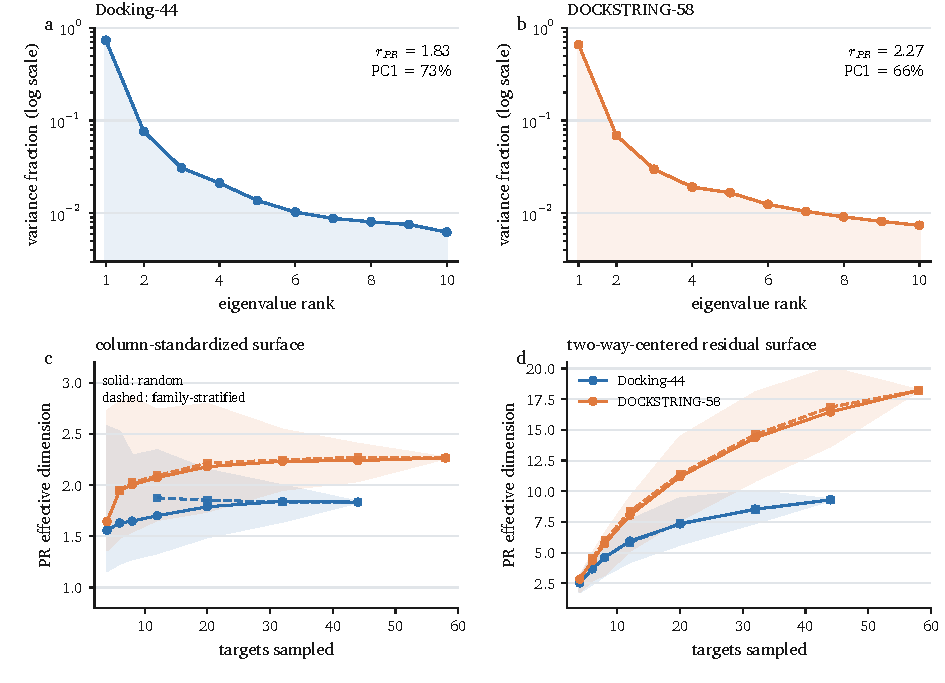
\includegraphics{figures/fig1_raw_collapse.pdf}
\caption{\textbf{Two independent Vina panels have concentrated column-standardized spectra.}
\textbf{a,b}, Eigenvalue spectra and PR effective dimensions of the
44-target antitarget and 58-target DOCKSTRING matrices after column standardization.
\textbf{c,d}, Column-standardized and two-way-centered residual PR effective dimensions
under target subsampling. Solid lines and shaded 2.5--97.5\% intervals show 200 uniform
subsets; dashed square-marked lines show 200 family-stratified subsets where the requested
size permits representation of every broad family. Full-panel points use all ligands.}
\label{fig:raw}
\end{figure}

\subsection{The leading direction is a shared docking-score axis}

The dominant direction was shared across targets rather than localized to one receptor
family. After orienting principal component 1 (PC1) consistently, 43 of 44 Docking-44
loadings and 57 of 58 DOCKSTRING loadings were positive (Fig.~\ref{fig:axis}c,d). The PC1
scores correlated 0.997 and 0.995 with the corresponding per-ligand mean of the original
score matrix. These are raw score-scale row means, not means calculated after column
standardization. Seven physicochemical descriptors explained 60.6\% of the variance in the
Docking-44 row mean; heavy-atom count alone explained 18\%.

Removing size-related information weakened but did not erase the concentration. Linear
residualization of each target score against seven physicochemical descriptors increased
$r_{\mathrm{PR}}$ from 1.83 to 2.54; cross-fitted nonlinear residualization increased it to
3.52. Restricting the data to 4,308 molecules with 17--22 heavy atoms still gave PR
dimension 1.70. Dividing scores by heavy-atom count made the spectrum more concentrated
(PR dimension 1.14), showing
that ligand-efficiency normalization is not a dimensionality correction. Across 36 targets,
pocket volume correlated 0.514 (target bootstrap interval 0.272--0.686) with the absolute
correlation between each target and the per-ligand panel mean. A 13-descriptor pocket model
had negative leave-one-target-out $R^2$ for both ordinary least squares ($-0.011$) and ridge
regression ($-0.144$), so the data do not support a multivariable pocket-mechanism claim. On the exact 74-by-6
experimental support, linear and five-fold cross-fitted nonlinear descriptor residualization
raised docking PR dimension only to 2.81 and 2.68, respectively, still below the
exact-relation median experimental value of 3.83. Thus the matched contrast is not solely a
consequence of the seven measured
bulk descriptors.

\begin{figure}[htbp]
\centering
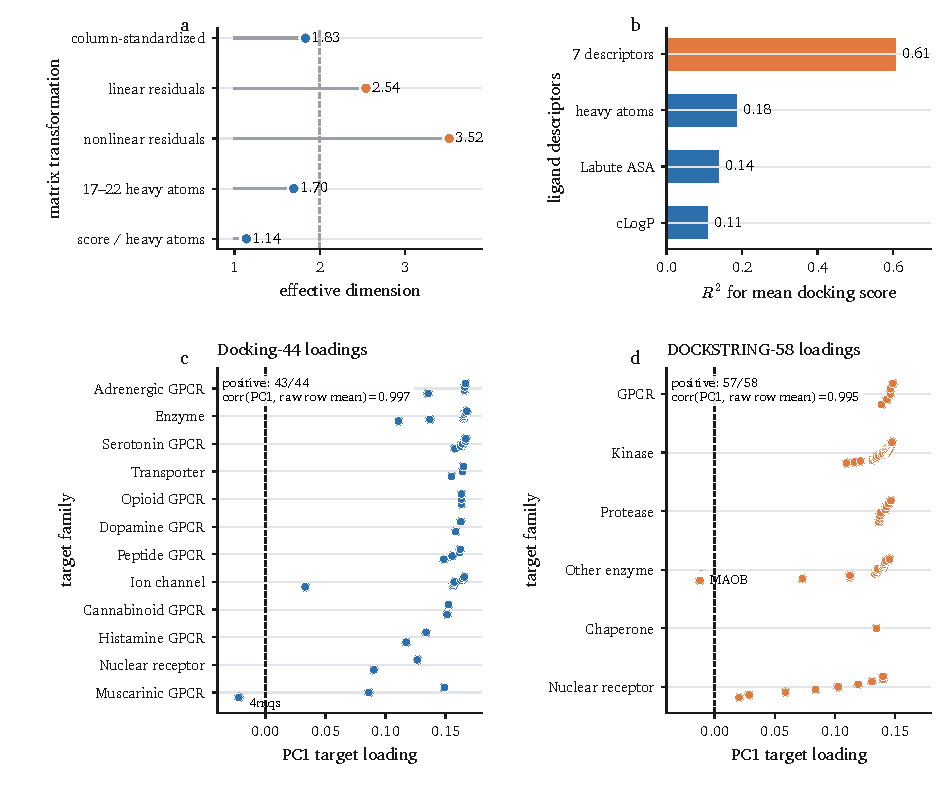
\includegraphics{figures/fig2_shared_axis.pdf}
\caption{\textbf{The leading component is a shared docking-score axis.}
\textbf{a}, Docking-44 PR effective dimension after physicochemical transformations;
the horizontal segments connect each estimate to one and are visual guides, not confidence
intervals. \textbf{b}, Variance in the raw per-ligand mean score explained by seven ligand
descriptors and single-descriptor controls. \textbf{c,d}, PC1 target loadings grouped by
curated target family. Loading signs were oriented so that the majority are positive. The
annotations report the number of positive loadings and the correlation between PC1 scores
and raw per-ligand mean scores. Descriptor residualization is diagnostic and is not proposed
as a scoring function.}
\label{fig:axis}
\end{figure}

\subsection{The docking--experiment contrast narrows after centering}

A concentrated docking surface could reflect its compounds or targets rather than its score
model. We therefore used the same 74 compounds and six aminergic targets for docking and
ChEMBL. The primary experimental curation required an exact standard relation, retained Ki,
Kd, IC50 and EC50, aggregated repeated compound--target activities by the median, and
required measurements for at least five of six targets. Target-median imputation filled
9.9\% of cells. The resulting ChEMBL surface had PR dimension 3.833, compared with 1.827 for
docking on the same support (Fig.~\ref{fig:matched}a). The paired ligand-bootstrap interval
for the experimental-minus-docking difference of 2.006 was 1.174--2.673.

The comparison changed in the residual space. After two-way centering, the docking and
experimental PR dimensions were 3.646 and 4.128. Their difference was 0.483, with a paired
bootstrap interval of $-0.071$--0.921 (Fig.~\ref{fig:matched}b). Thus, much of the raw
docking--experiment contrast on this support arose from the shared ligand direction. It did
not persist as a clearly resolved difference between residual effective dimensions.

Multiple imputation supported the same qualitative reading. Across 100 posterior chained-
regression imputations, the median experimental PR dimensions were 3.823 before centering
and 4.069 afterward. The corresponding experimental-minus-docking differences had medians
1.996 and 0.423. The displayed 95\% ranges across imputations quantify missing-value
sensitivity; they are not bootstrap confidence intervals.

More restrictive assay blocks preserved the ordering. Human binding assays with all four
endpoints gave 3.510 for ChEMBL and 1.865 for docking on 47 ligands. Restricting further to
human binding Ki/Kd gave 3.072 and 1.894 on 35 ligands. These comparisons do not define the
dimension of experimental binding in general: the assays come from multiple laboratories
and conditions, up to 13.3\% of cells are imputed, and six targets cap the centered
algebraic dimension at five. They support only the statement that these matched ChEMBL
surfaces are less spectrally concentrated than docking on the same ligand--target support.

Additional controls addressed assay choice, missingness and measurement heterogeneity. A fully observed
31-by-6 ChEMBL sub-block had PR dimension 3.61. On a secondary 212-by-22 block, estimates
were 5.72 with K-nearest-neighbour imputation, 8.59 averaged over chained imputations, 2.64
with low-rank matrix completion and 7.28 with probabilistic-PCA expectation maximization;
the magnitude depended on the estimator. A separate frozen ChEMBL extraction with the same
nominal 212-by-22 shape and 52.9\% missingness gave KNN PR dimension 6.85; we retain both in
Supplementary Table~S3 as a curation-sensitivity discrepancy. A legacy most-potent aggregation of the 74-by-6
block gave 3.734 for experiment and 1.827 for docking, with a paired bootstrap difference
interval of 1.05--2.61, and is retained only as a sensitivity. Different-document repeats
estimated a standard deviation of 0.493 pChEMBL units. Adding target-scaled Gaussian noise
at that level to docking raised its median PR dimension to 2.29 (simulation interval
2.12--2.50); approximately 2.5 times that scale was required to reach the legacy
experimental value. None of these controls removes all biological, laboratory or
condition-related heterogeneity.

\begin{figure}[htbp]
\centering
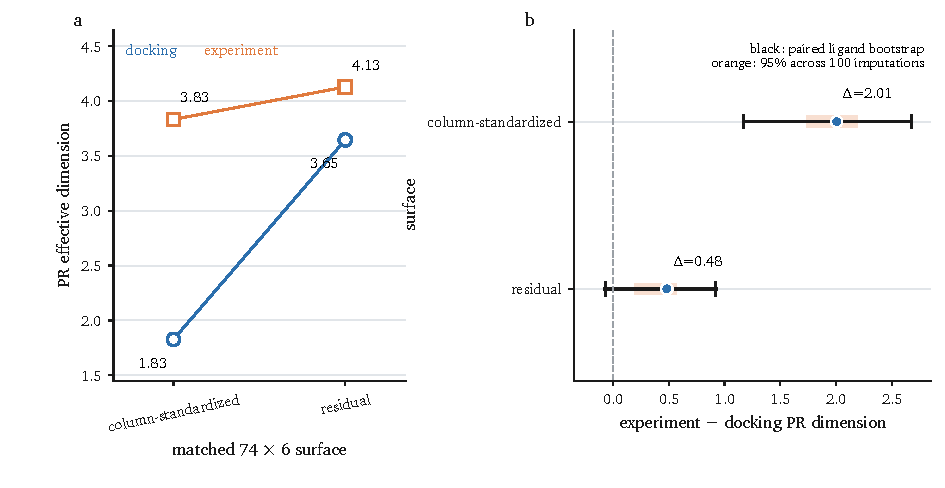
\includegraphics{figures/fig3_matched_experiment.pdf}
\caption{\textbf{The matched docking--experiment contrast is mainly a raw-surface
contrast.} \textbf{a}, PR effective dimensions for docking and exact-relation median ChEMBL
on the same 74 compounds and six targets, before and after two-way centering. \textbf{b},
Experimental-minus-docking differences. Black intervals are paired ligand-bootstrap 95\%
intervals; orange bands are the central 95\% of the difference across 100 posterior multiple
imputations. These intervals answer different uncertainty questions and are not pooled.}
\label{fig:matched}
\end{figure}

\subsection{Centering reveals higher-dimensional but still concentrated residual surfaces}

The column-standardized spectrum mixes the ligand main effect with the ligand--target
residual. We removed both row and column means according to Eq.~\ref{eq:decomposition} and
then applied the same column standardization and spectral estimator. This changed the
measured object and the answer (Fig.~\ref{fig:centering}a). Docking-44 rose from PR dimension
1.834 to 9.303; a paired Butina-cluster bootstrap placed the increase at 6.982--7.909.
DOCKSTRING rose from 2.266 to 18.206, and five independent 15,000-molecule supports gave
increases from 15.880 to 16.045. The corresponding PC1 fractions fell from 73.3\% to 27.4\%
and from 65.9\% to 17.8\%. In unstandardized sum-of-squares terms, the residual retained
27\% and 31\% of grand-centered variation. Low variance relative to a main effect is not
absence.

The increase was not only a rescaling artifact of the PR denominator. Relative to the
available algebraic maximum, normalized PR dimensions increased from 0.042 ($1.834/44$) to 0.216 ($9.303/43$)
for Docking-44 and from 0.039 ($2.266/58$) to 0.319 ($18.206/57$) for DOCKSTRING.
This normalization is a ceiling reference, not a correction for target count: the residual
PR dimension increased with panel size while its ratio to $P-1$ decreased
(Fig.~\ref{fig:raw}d). At a matched 44 targets, the DOCKSTRING median residual PR dimension
was 16.47 (target-subset interval 13.72--20.03), compared with 9.30 for the full Docking-44
panel. The cross-dataset difference therefore remained at matched $P$, although part of the
18.21-versus-9.30 contrast reflects different target counts.

Higher-dimensional did not mean unconcentrated. We fitted an additive null retaining the
observed grand mean, ligand effects, target effects and target-specific residual variances,
but drawing residuals independently. After two-way centering, its median PR dimensions were
42.40 for Docking-44 and 56.48 for DOCKSTRING, close to the respective $P-1$ ceilings of 43
and 57. The observed residual values, 9.29 and 18.16 on the same 12,000-row supports, were
smaller than every one of 500 null realizations (one-sided empirical $p=0.002$ for each;
Fig.~\ref{fig:centering}b). Centering therefore exposes more residual directions, while the
residual correlations remain far stronger than independent-noise expectations.

In the transformation-matched permutation analysis, the descriptive rank-wise mode counts
increased from 3 to 7 and from 4 to 10. The same counts survived the simultaneous
studentized maximum-deviation envelope and were unchanged in five independent 100-
permutation series. Because even weak correlations can become statistically detectable at
large sample size, we use these counts to describe spectrum shape rather than as a measure
of practical dimension.

Two-way centering also creates an exact structural constraint: every interaction row sums
to zero. Non-zero column scaling preserves one linear dependence, so the interaction matrix
has algebraic rank at most $P-1$ and one correlation eigenvalue is zero. Residual and
column-standardized PR dimensions therefore describe different constrained spaces; the centered increases
occur despite, not because of, a larger algebraic maximum.

\begin{figure}[htbp]
\centering
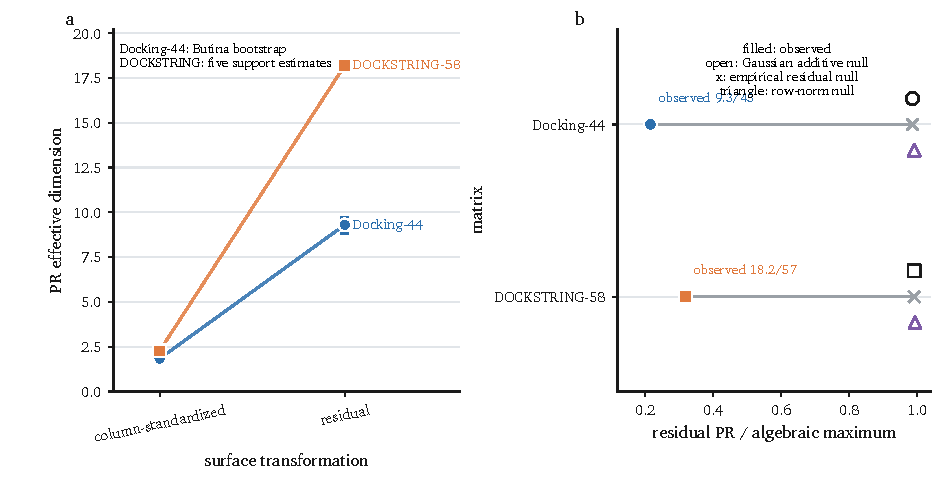
\includegraphics{figures/fig4_centering_null.pdf}
\caption{\textbf{Two-way centering increases effective dimension without removing residual
concentration.} \textbf{a}, Paired raw-to-residual changes. Docking-44 error bars are 95\%
Butina-cluster bootstrap intervals; DOCKSTRING error bars span point estimates across five
independently seeded 15,000-molecule supports. \textbf{b}, Observed residual PR dimensions
and fitted additive-null medians, each divided by its $P-1$ algebraic maximum. Open-marker
bars are the central 95\% of 500 null realizations and are visually narrower than the marker.
The null preserves fitted ligand and target effects and target-specific residual variance,
but removes cross-target residual dependence.}
\label{fig:centering}
\end{figure}

\subsection{Higher residual dimension does not by itself improve target ranking}

We evaluated an operational reverse-docking endpoint on the primary matched ChEMBL support.
For each ligand, every observed pair of targets with unequal experimental pChEMBL values was
scored as correctly ordered or not. Target offsets and scales were estimated leave-one-
ligand-out, so the evaluated ligand did not contribute to its transformation. The primary
mean gave equal weight to each of 74 ligands; 887 target pairs were evaluated and three
exact experimental ties were excluded.

Absolute Vina scores reached mean pairwise target-preference accuracy 0.619, with a
scaffold-cluster bootstrap interval of 0.566--0.673 (Fig.~\ref{fig:preference}a). This did not
establish ligand-specific target recognition. A target-offset-only baseline, which assigns
the same target order to every held-out ligand, reached 0.625 (0.580--0.668). The paired
absolute-score minus target-only difference was $-0.006$ ($-0.040$--0.028). Moreover,
permuting ligand identities within each target produced mean accuracy 0.624 and reproduced
or exceeded the observed absolute-score result in 63.8\% of 5,000 permutations. Across the
six targets, favorable mean Vina score and mean observed pChEMBL were aligned
($r_s=0.77$; Fig.~\ref{fig:preference}b). The apparent absolute-score performance is thus
consistent with target-level affinity priors rather than resolved evidence of within-ligand
target specificity.

Column standardization removed much of this target prior and gave accuracy 0.537
(0.495--0.575); two-way residualization gave 0.540 (0.497--0.584). Their paired difference
was 0.004, with a scaffold-cluster interval of $-0.019$--0.026. The normal-approximation
minimum detectable difference for 80\% power was about 0.030, so the data exclude neither a
smaller benefit nor a smaller harm. Two-way residualization was also 0.079 below the
absolute-score result ($-0.119$--$-0.039$), even though it had the higher PR dimension. Pair-
weighted summaries, a 0.10-pChEMBL tie tolerance and 100 multiple imputations gave the same
qualitative ordering (Supplementary Table~S5).

This negative comparison supplies the operational boundary of the spectral analysis.
Two-way centering answers whether ligand and target main effects conceal structured residual
variation. It does not determine whether that variation orders targets correctly. A reverse-
docking workflow should therefore report target-only and ligand-shuffle baselines and choose
its score transformation by external task-level validation, not by effective dimension
alone.

\begin{figure}[htbp]
\centering
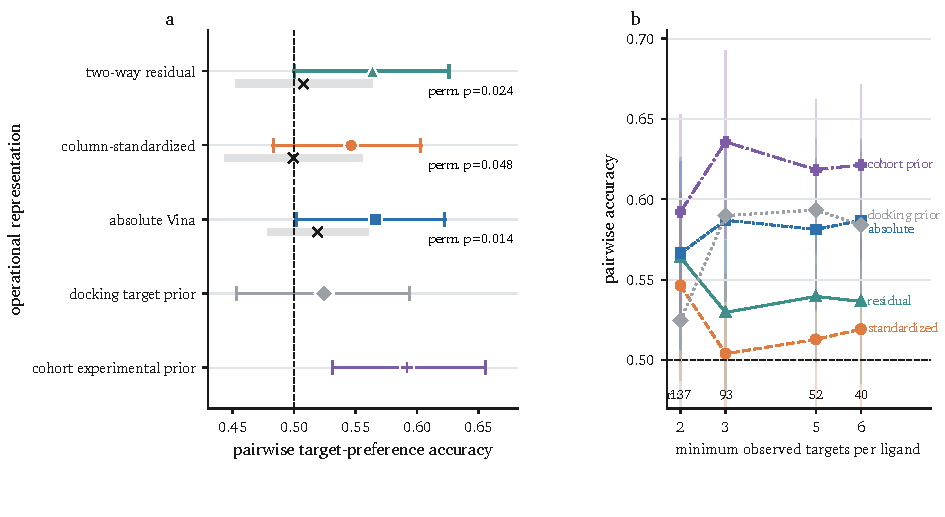
\includegraphics{figures/fig5_target_preference.pdf}
\caption{\textbf{Spectral and operational conclusions are distinct.}
\textbf{a}, Leave-one-ligand-out pairwise target-preference accuracy on observed cells of the
matched 74-by-6 ChEMBL support. Colored intervals are 95\% scaffold-cluster bootstrap
intervals. Grey bars and crosses show the central 95\% and mean of 5,000 ligand-identity
permutations; labels give one-sided empirical probabilities. The dashed line is chance.
\textbf{b}, Target-level mean alignment between favorable Vina score and observed pChEMBL;
target identifiers are shown because only six targets are available.}
\label{fig:preference}
\end{figure}

\section{Discussion}

The two large Vina panels share a concentrated column-standardized spectrum, but centering
does not make the residuals unconcentrated. The raw PR dimensions of 1.83 and 2.27 rose to
9.30 and 18.21 after ligand and target main effects were removed; the fitted additive nulls,
however, placed independent residual noise near 42 and 56 dimensions. The empirical
residuals therefore contain more directions than the shared-score surface while remaining
strongly correlated. The result is a reduction in spectral concentration, not its
disappearance.

Two-way normalization and PCA themselves predate this work. SePreSA used two-directional
normalization of docking-score matrices, and earlier protein--compound affinity work used
principal components as multidimensional descriptors.\cite{sepresa2009,fukunishi2006,fukunishi2018}
Our contribution is the quantitative separation of raw and residual spectral
estimands on two large dense panels, uncertainty with respect to target and chemical
composition, and an operational test of whether the richer residual spectrum improves
target ranking.

The loading analysis explains why the estimands diverge. Almost every target loaded in the
same direction on PC1, and PC1 scores were nearly identical to the raw per-ligand mean score.
Ligand bulk accounted for part, but not all, of this direction. Column standardization
removes target offsets while retaining the shared ligand tendency; two-way centering removes
that tendency and reveals the remaining cross-target covariance. We call this a shared
docking-score axis rather than a general-binding axis because neither its biological meaning
nor universal validity was established.

On the matched ChEMBL support, experimental affinities were
less concentrated than docking before centering, but the paired residual-space difference
was smaller and its bootstrap interval included zero. This does not show that Vina residuals
reproduce experimental geometry. It shows that the raw docking--experiment contrast on this
support is largely a contrast in shared main effects rather than a resolved difference in
residual PR dimension.

Operational validation changed the interpretation again. Absolute Vina scores appeared
to rank experimental target preferences above chance, yet a target-only ordering performed
as well and ligand shuffling reproduced the result. The six targets differed systematically
in both mean Vina score and mean ChEMBL activity, allowing a method to achieve apparent
accuracy without resolving which target a particular ligand preferred. Removing target
offsets removed this source of performance, but two-way residualization did not improve on
column standardization. Higher residual dimension is therefore neither necessary nor
sufficient for a useful reverse-docking score.

Accordingly, a spectral audit should report both the
column-standardized and two-way-centered spectra, transformation-matched nulls and the
chemical and target populations represented by its uncertainty. A reverse-docking
benchmark should additionally include a target-only prior and a ligand-identity-shuffle
null. The operational score representation should be selected on held-out experimental
target preferences. Two-way centering can be retained as a diagnostic even when it is not
the selected ranking rule.

Both large matrices use Vina-family scores, and the small RF-Score blocks in Supplementary
Fig.~S3 cannot represent modern learned scoring
functions. Neither target panel is a probability sample from all pharmacologically relevant
proteins, so jackknife and family-stratified subsampling quantify stability within the
observed panels. The downstream benchmark contains only 74 ligands and six aminergic
targets, has 9.9\% missing experimental cells, and has about 80\% power only for paired
accuracy changes of approximately 0.03 or larger. Multiple imputation, scaffold resampling
and tie sensitivity address parts of this uncertainty but do not enlarge its biological
scope. Finally, the public package reproduces analysis from frozen matrices; it does not
rerun upstream receptor preparation, docking, pose generation or RF-Score rescoring.

\section{Conclusions}

Two-way centering reveals substantially higher-dimensional residual structure in two
spectrally concentrated Vina matrices, but the residuals remain far more concentrated than
an additive independent-noise null. On matched ChEMBL data, the transformation narrowed the
docking--experiment PR contrast without improving target-preference accuracy over column
standardization. The practical consequence is to separate diagnosis from correction:
spectral analysis can identify shared ligand and target effects, whereas a score
transformation for reverse docking must earn its use against target-only and ligand-shuffle
baselines on held-out experimental data.

\section{Methods}

\subsection{Datasets and score panels}

The antitarget matrix was taken from the open resource of Nikitin et al.\cite{nikitin2025}
and contained 12,651 analyzable compounds and 44 Vina-GPU target
scores.\cite{vina2010} The source pipeline clipped positive scores to zero; its processed
matrix contained 111 such zero-censored cells (0.020\%) and no remaining positive values.
Missing entries comprised 1.466\% of cells and were replaced by the target mean for the
primary analysis. Chemical-cluster uncertainty used the precomputed 8,150 Butina clusters
supplied with the dataset. A three-target Docking-47 expansion is reported only as an
illustrative sensitivity in the Supplement.

DOCKSTRING was read from its released full score table.\cite{dockstring2022} We used the 58
target columns, clipped positive scores to zero for consistency and used the 260,060 rows
with complete scores for the primary spectrum. Only 0.0022\% of entries were missing and
0.0358\% were positive before clipping; an unclipped sensitivity retained these values.

RF-Score v1 was evaluated with the Open Drug Discovery Toolkit implementation.\cite{rfscore2010,oddt}
The first panel comprised the 41 ligands complete across RF-Score, smina/Vina and original
Vina scores for 14 targets. The second comprised 35 ligands complete across RF-Score on
Vinardo poses and original Vina scores for 20 targets. These are scoring-function and
pose-source sensitivities, not affinity benchmarks, and are reported with the Docking-47
expansion in Supplementary Fig.~S3.

Experimental activities came from ChEMBL release 34.\cite{mendez2019} We retained records
with a pChEMBL value and standard type Ki, Kd, IC50 or EC50; canonical SMILES were converted
to full InChIKeys and targets were mapped to the panel's single-protein accessions. The
primary matched block was rebuilt from activity-level records, required an exact standard
relation and full InChIKey, and aggregated repeated compound--target activities by the
median. It used 74 compounds with docking scores for six targets and ChEMBL measurements for
at least five targets; 9.9\% of experimental cells were median-imputed within target. We
additionally restricted to human binding assays, either with all four
endpoints or with Ki/Kd only. A secondary 212-by-22 block required at least eight measured
targets per ligand and 30 measurements per retained target. We compared five-nearest-neighbor
imputation, multiple imputation by chained equations, low-rank matrix completion and
probabilistic-PCA expectation maximization. Assay sensitivity separately retained binding
records with Ki or Kd endpoints from the already human-only curated refetch. Relations
reported as inequalities and records
without pChEMBL were excluded. A frozen table that retained the most potent pChEMBL value per
compound--target pair was analyzed only as a legacy sensitivity with a paired ligand
bootstrap.

DAVIS experimental affinity\cite{davis2011} and Boltz-2\cite{boltz2} were read from versioned matrices in
the release only for a contextual centering ladder in Supplementary Fig.~S4. The common
surface contained 72 ligands and 442 kinases. PR dimensions were computed on each complete
dense matrix, including pKd-floor values, because the surfaces were aligned. The exploratory
rank--selectivity analysis is reported entirely in the Supplement; its complete panel has 20
arms, while the 12-arm above-chance subset is an outcome-restricted sensitivity.

\subsection{Spectral quantities}

For each complete matrix $X$, columns with zero variance were removed and the remaining
columns were standardized to zero mean and unit sample variance, producing $Z$. We formed
the target correlation matrix
\begin{equation}
C=\frac{1}{N-1}Z^{\mathsf T}Z
\end{equation}
and sorted its non-negative eigenvalues $\lambda_1\geq\cdots\geq\lambda_P$. The primary
summary was the PR effective dimension in Eq.~\ref{eq:pr}. We also computed the entropy rank
$\exp[-\sum_k p_k\log p_k]$, where $p_k=\lambda_k/\sum_l\lambda_l$, the fraction explained
by principal component 1 and the number of components reaching 80\% and 90\% cumulative
variance. Equation~\ref{eq:prcorr} follows from
$\operatorname{tr}(C^2)=P+P(P-1)\overline{r_{ij}^{\,2}}$. The PR effective dimension is especially
sensitive to dominant eigenvalues, whereas entropy rank weights the spectral tail more
strongly. Both are continuous summaries of variance concentration, not algebraic or
nonlinear manifold ranks.

The Marchenko--Pastur upper edge $(1+\sqrt{P/N})^2$ was used as an asymptotic guide. The
original panel analyses anchored mode counts on column-wise permutation parallel analysis,
which preserves each score marginal while breaking cross-target alignment.\cite{horn1965}
For direct column-standardized--residual comparison, we additionally drew the same 12,000
rows from each large matrix, generated 500 independent column-wise permutations, applied
either no centering or two-way centering to both observed and permuted matrices, and counted
observed eigenvalues above the rank-wise 95th percentile of the corresponding null. Because
rank-wise comparisons do not control multiplicity, we also formed a 95\% simultaneous
envelope from the maximum studentized deviation over all eigenvalue ranks. Rank-wise counts
are treated as descriptive; the simultaneous envelope controls the family-wise error rate.
We repeated the count in five independent 100-permutation series to assess Monte Carlo
stability.
The 44-target analysis additionally used cluster-preserving and cluster-representative nulls;
the latter retained three leading modes and controlled the inflated false-positive rate
caused by chemical clustering. Effective-dimension intervals and the paired raw-to-residual
difference for that panel resampled Butina clusters 500 times. DOCKSTRING used 100 molecule
and 100 Bemis--Murcko scaffold-cluster replicates on each of five independently seeded
15,000-row supports. The primary matched experiment used a paired ligand bootstrap. These
intervals are conditional on the observed target panels; chemical resampling does not
represent target-selection uncertainty.

\subsection{Main-effect removal}

For complete matrices we computed the interaction residual in one closed-form step,
\begin{equation}
\Gamma=X-\bar X_{\cdot j}-\bar X_{i\cdot}+\bar X_{\cdot\cdot},
\end{equation}
where the bars denote column, row and grand means. We then column-standardized $\Gamma$ and
computed exactly the same spectral summaries. Because standardization already removes column
offsets, the change from the column-standardized to residual spectra is driven principally by removal of the
per-ligand common direction. The fraction of grand-centered unstandardized sums of squares
retained by $\Gamma$ was reported separately and was not used as a PR-dimension measure.
Each row of $\Gamma$ sums to zero. Subsequent non-zero column scaling preserves one exact
linear dependence, so $\operatorname{rank}(\Gamma)\leq P-1$ and the residual correlation
spectrum contains one structural zero eigenvalue. For an additive model with independent,
identically distributed residual noise, the non-zero residual spectrum is flat and the PR
dimension approaches $P-1$. We therefore treat $P-1$ as a noise ceiling, not as a
panel-size correction, and show target-subsampling curves for the residual estimand.

To test whether centering alone mechanically produced the observed residual spectra, we fit
the additive model in Eq.~\ref{eq:decomposition} on a common 12,000-row support. For each of
500 realizations, residuals were drawn independently from zero-mean Gaussian distributions
with the observed target-specific residual variances, then added to the fitted grand,
ligand and target effects. We two-way centered each simulated matrix and recomputed PR
dimension. The one-sided empirical probability was calculated with the finite-simulation
correction $(1+k)/(1+500)$, where $k$ is the number of null PR dimensions no larger than the
observed value.

\subsection{Physicochemical-axis analyses}

The full-panel and matched-support residualizations used seven RDKit descriptors: heavy-atom
count, molecular weight, Labute accessible surface area, topological polar surface area,
Crippen cLogP, rotatable-bond count and ring count. Descriptors were standardized. For the full antitarget panel, a separate
ordinary least-squares model was fit for each target and residuals were assembled before
spectral analysis. The nonlinear sensitivity used five-fold shuffled cross-fitting (seed 0)
with one histogram gradient-boosting regressor per target (200 iterations, learning rate
0.05, maximum depth 4); no ligand's fitted value came from a model trained on that ligand.
The same protocol was repeated on the matched 74-by-6 support. The narrow-size sensitivity
retained molecules with 17--22 heavy atoms, and ligand efficiency divided each score by
heavy-atom count. A separate cached diagnostic of the shared score direction used molecular
weight, cLogP, topological polar surface area, hydrogen-bond donor and acceptor counts,
rotatable-bond count and molecular volume. Pocket volumes were read from the frozen
44-pocket structure summary; 36 targets had complete volumes. The reported univariate
statistic correlates pocket volume with the absolute correlation between each target score
and the per-ligand panel mean, not with a principal-component loading. The 13-descriptor
pocket model was evaluated by leave-one-target-out prediction.

\subsection{Preprocessing and experimental-noise sensitivities}

For the antitarget panel we repeated the column-standardized analysis with target-median imputation
($r_{\mathrm{PR}}=1.835$), complete cases (9,297 ligands; 1.320), pairwise-complete Pearson
correlations (1.788) and pairwise Spearman correlations (1.686). The complete-case estimate
changes the chemical support and is not a like-for-like imputation test. Censoring
sensitivities treated source-clipped zero cells as missing, removed every affected ligand or
removed the most affected target decile. For interaction spectra we compared
score-scale centering followed by standardization (9.303), standardization followed by
centering (9.378), and robust median/interquartile-range scaling followed by centering
(9.462). These analyses test analysis-pipeline sensitivity rather than define alternative
primary endpoints.

For the primary 74-by-6 ChEMBL block, target-median imputation was supplemented by 100
posterior multiple imputations from chained Bayesian-ridge regressions. Imputed values were
bounded by the observed range of each target. We recomputed both raw and residual PR
dimensions and all downstream preference metrics in every completed matrix. Central 95\%
ranges across imputations describe missing-value sensitivity and are not interpreted as
frequentist confidence intervals.

Different-document ChEMBL repeats for the same compound--target pair provided a conservative
repeatability scale. From 279,012 paired records, the median absolute difference was 0.47
pChEMBL and the implied single-measurement Gaussian standard deviation was 0.493. For each
of the six matched targets, this standard deviation was divided by that target's experimental
standard deviation. Independent Gaussian noise at the resulting target-specific scales was
added to the standardized docking block in 2,000 simulations before recomputing PR dimension. This
calibration includes inter-laboratory and condition variation; it is not a pure technical
replicate variance or a complete experimental noise model.

\subsection{Chemical- and target-composition sensitivities}

Target-subsampling curves used 200 subsets without replacement at each reported size on one
seeded 12,000-ligand support; the complete-panel points used all eligible ligands. Uniform
sampling was paired with broad family-stratified sampling based on the versioned
\path{data/target_families.csv} manifest. Stratified allocations were proportional to family
size and included at least one target from every family whenever the requested subset size
permitted. Both the column-standardized and two-way-centered residual PR dimensions were
recomputed after every draw.

Leave-one-target-out analysis used all 12,651 Docking-44 ligands and one seeded 15,000-row
DOCKSTRING support; complete-panel estimates on the same support were plotted as references.
The resulting minima, medians and maxima are composition sensitivities, not confidence
intervals for a target superpopulation. Ligand-subsampling curves used 50 subsets. For the
DOCKSTRING chemical-cluster sensitivity, Bemis--Murcko scaffolds were generated with RDKit;
acyclic molecules were treated as singletons. One hundred cluster-bootstrap replicates were
compared with 100 molecule-bootstrap replicates on each of five independent 15,000-molecule
supports. The first support used the prespecified seed 0; the remaining support seeds were
drawn reproducibly from that generator.

\subsection{Matched target-preference benchmark}

The operational endpoint used only observed exact-relation median ChEMBL cells in the
74-by-6 block. For each ligand and every pair of observed targets, a prediction was correct
when the more negative docking representation corresponded to the larger experimental
pChEMBL value. Exact pChEMBL ties were excluded. The primary statistic was the mean of per-
ligand pairwise accuracies, giving each ligand equal weight; pair-weighted accuracy, mean
within-ligand Spearman correlation and top-1 accuracy were secondary. The Vina energy sign
convention---more negative predicts stronger binding---was fixed before examining the
results.

Five operational representations were compared. Absolute Vina used the original scores. A
target-offset-only baseline assigned each held-out ligand the training-set target means.
Column-standardized scores used training-set target means and sample standard deviations.
Two-way residual scores additionally removed the held-out ligand's row mean and the
training grand mean, then divided by training residual target standard deviations. An
experimental target-prior reference ranked the training-set target mean pChEMBL values. All
target means, grand means and scale estimates were cross-fitted leave-one-ligand-out, so the
evaluated ligand did not contribute to its transformation.

Uncertainty was estimated by 5,000 ligand bootstraps and 5,000 Bemis--Murcko scaffold-
cluster bootstraps over 61 matched clusters. Paired comparisons resampled the per-ligand
accuracy difference. Ligand-identity nulls independently permuted rows of each score
representation relative to the experimental matrix 5,000 times; one-sided probabilities
used the finite-permutation correction. Sensitivities used pair weighting, a 0.10-pChEMBL
tie tolerance and the 100 completed multiple-imputation matrices. A normal-approximation
minimum detectable effect was reported for the paired residual-minus-column comparison at
two-sided $\alpha=0.05$ and 80\% power.

\subsection{Software and reproducibility}

The new analyses and figures were run with Python 3.12.11, NumPy 1.26.4, pandas 2.3.2,
SciPy 1.16.2, scikit-learn 1.7.2, Matplotlib 3.10.6 and RDKit 2025.03.6. The release's
\path{analysis/build_evidence.py} regenerates the centering ladder, preprocessing controls,
experimental sensitivities, subsampling results and DTI associations in
\path{results/evidence_summary.json}; it also embeds explicitly labelled summaries from the
frozen upstream docking/rescoring stages. \path{analysis/make_figures.py} regenerates all
main and supplementary figures. The core release reproduces the reported analysis from
frozen matrices and summaries; it does not rerun receptor preparation, docking or RF-Score
pose rescoring. A checksum manifest, pinned requirements, environment file,
Dockerfile and Makefile provide input verification and one-command regeneration. Random seed
0 initializes all stochastic procedures; derived support and replicate seeds are stored in
the evidence ledger.

OpenAI Codex and Anthropic Claude were used during manuscript preparation for code review,
literature-search assistance and language editing. They were not treated as sources of
scientific evidence. The authors inspected the underlying data and code, verified the
reported claims and citations, and retain responsibility for the work.

\section*{List of abbreviations}

DTI, drug--target interaction; KNN, k-nearest neighbors; PC, principal component; RMT,
random matrix theory; PR, participation ratio.

\section*{Declarations}

\subsection*{Ethics approval and consent to participate}

Not applicable.

\subsection*{Consent for publication}

Not applicable.

\subsection*{Availability of data and materials}

The source antitarget dataset is available with Nikitin et al.\cite{nikitin2025}; DOCKSTRING
scores and poses are available from the DOCKSTRING release.\cite{dockstring2022} DAVIS and
ChEMBL are publicly available from their respective source repositories. The derived
matrices, frozen summaries, source manifest and analysis code are available without
registration under an OSI-approved code license in the versioned GitHub repository and
Zenodo archive.\cite{softwaregithub,softwarezenodo} The exact submission package corresponds
to GitHub tag \path{v1.1.0}. Upstream datasets retain their stated licenses and are identified
by source URL, version and checksum in the manifest.

\subsection*{Competing interests}

The authors declare that they have no competing interests.

\subsection*{Funding}

This research received no specific grant from any funding agency in the public, commercial,
or not-for-profit sectors.

\subsection*{Authors' contributions}

A.L. conceived the study, performed the analyses and drafted the manuscript. V.S. and M.F.
contributed to study design and interpretation. All authors reviewed the manuscript and are
responsible for the final submitted version.

\subsection*{Acknowledgements}

The authors thank the developers and maintainers of the open datasets and software used in
this study.

\subsection*{Authors' information}

ORCID: Adeliya Leleytner, 0009-0001-8214-2496; Victor Safronov,
0009-0003-5668-0201; Maxim Fedorov, 0000-0003-3901-3565.

\begin{thebibliography}{99}
\small

\bibitem{sepresa2009} Yang L, Luo H, Chen J, Xing Q, He L (2009) SePreSA: a server for
the prediction of populations susceptible to serious adverse drug reactions implementing
the methodology of a chemical--protein interactome. Nucleic Acids Res 37:W406--W412.
doi:10.1093/nar/gkp312.

\bibitem{fukunishi2006} Fukunishi Y, Mikami Y, Takedomi K, Yamanouchi M, Shima H,
Nakamura H (2006) Classification of chemical compounds by protein--compound docking for use
in designing a focused library. J Med Chem 49:523--533. doi:10.1021/jm050480a.

\bibitem{fukunishi2018} Fukunishi Y, Yamashita Y, Mashimo T, Nakamura H (2018)
Prediction of protein--compound binding energies from known activity data: docking-score-based
method and its applications. Mol Inform 37:e1700120. doi:10.1002/minf.201700120.

\bibitem{pan2003} Pan Y, Huang N, Cho S, MacKerell AD Jr (2003) Consideration of
molecular weight during compound selection in virtual target-based database screening.
J Chem Inf Comput Sci 43:267--272. doi:10.1021/ci020055f.

\bibitem{jacobsson2006} Jacobsson M, Karl\'en A (2006) Ligand bias of scoring functions in
structure-based virtual screening. J Chem Inf Model 46:1334--1343.
doi:10.1021/ci050407t.

\bibitem{carta2007} Carta G, Knox AJS, Lloyd DG (2007) Unbiasing scoring functions: a new
normalization and rescoring strategy. J Chem Inf Model 47:1564--1571.
doi:10.1021/ci600471m.

\bibitem{luo2017} Luo Q, Zhao L, Hu J, Jin H, Liu Z, Zhang L (2017) The scoring bias in
reverse docking and the score normalization strategy to improve success rate of target
fishing. PLoS One 12:e0171433. doi:10.1371/journal.pone.0171433.

\bibitem{warren2006} Warren GL et al (2006) A critical assessment of docking programs and
scoring functions. J Med Chem 49:5912--5931. doi:10.1021/jm050362n.

\bibitem{dockstring2022} Garc\'ia-Orteg\'on M, Simm GNC, Tripp AJ,
Hern\'andez-Lobato JM, Bender A, Bacallado S (2022) DOCKSTRING: easy molecular docking
yields better benchmarks for ligand design. J Chem Inf Model 62:3486--3502.
doi:10.1021/acs.jcim.1c01334.

\bibitem{nikitin2025} Nikitin I, Morgunov I, Safronov V, Kalyuzhnaya A, Fedorov M
(2025) Towards explainable computational toxicology: linking antitargets to rodent acute
toxicity. Pharmaceutics 17:1573. doi:10.3390/pharmaceutics17121573.

\bibitem{rfscore2010} Ballester PJ, Mitchell JBO (2010) A machine learning approach to
predicting protein--ligand binding affinity with applications to molecular docking.
Bioinformatics 26:1169--1175. doi:10.1093/bioinformatics/btq112.

\bibitem{boltz2} Passaro S, Corso G, Wohlwend J et al (2025) Boltz-2: towards accurate and
efficient binding affinity prediction. bioRxiv. doi:10.1101/2025.06.14.659707.

\bibitem{davis2011} Davis MI, Hunt JP, Herrgard S et al (2011) Comprehensive analysis of
kinase inhibitor selectivity. Nat Biotechnol 29:1046--1051. doi:10.1038/nbt.1990.

\bibitem{oddt} W\'ojcikowski M, Zielenkiewicz P, Siedlecki P (2015) Open Drug Discovery
Toolkit (ODDT): a new open-source player in the drug discovery field. J Cheminform 7:26.
doi:10.1186/s13321-015-0078-2.

\bibitem{horn1965} Horn JL (1965) A rationale and test for the number of factors in factor
analysis. Psychometrika 30:179--185. doi:10.1007/BF02289447.

\bibitem{vina2010} Trott O, Olson AJ (2010) AutoDock Vina: improving the speed and
accuracy of docking with a new scoring function, efficient optimization, and
multithreading. J Comput Chem 31:455--461. doi:10.1002/jcc.21334.

\bibitem{gonen2012} G\"onen M (2012) Predicting drug--target interactions from chemical
and genomic kernels using Bayesian matrix factorization. Bioinformatics 28:2304--2310.
doi:10.1093/bioinformatics/bts360.

\bibitem{cobanoglu2013} Cobanoglu MC, Liu C, Hu F, Oltvai ZN, Bahar I (2013)
Predicting drug--target interactions from drug structure and protein sequence using
probabilistic matrix factorization. J Chem Inf Model 53:3399--3409.
doi:10.1021/ci400219z.

\bibitem{liu2016} Liu Y, Wu M, Miao C, Zhao P, Li X-L (2016) Neighborhood regularized
logistic matrix factorization for drug--target interaction prediction. PLoS Comput Biol
12:e1004760. doi:10.1371/journal.pcbi.1004760.

\bibitem{lee2016} Lee AA, Brenner MP, Colwell LJ (2016) Predicting protein--ligand
affinity with a random matrix framework. Proc Natl Acad Sci USA 113:13564--13569.
doi:10.1073/pnas.1611138113.

\bibitem{roy2007} Roy O, Vetterli M (2007) The effective rank: a measure of effective
dimensionality. In: 15th European Signal Processing Conference, Pozna\'n, pp 606--610.

\bibitem{mendez2019} Mendez D, Gaulton A, Bento AP et al (2019) ChEMBL: towards direct
deposition of bioassay data. Nucleic Acids Res 47:D930--D940.
doi:10.1093/nar/gky1075.

\bibitem{graczyk2007} Graczyk PP (2007) Gini coefficient: a new way to express
selectivity of kinase inhibitors against a family of kinases. J Med Chem 50:5773--5779.
doi:10.1021/jm070562u.

\bibitem{bosc2017} Bosc N, Meyer C, Bonnet P (2017) The use of novel selectivity metrics
in kinase research. BMC Bioinformatics 18:17. doi:10.1186/s12859-016-1413-y.

\bibitem{softwaregithub} Leleytner A, Safronov V, Fedorov M (2026) Spectral concentration
in Vina docking-score matrices: analysis code and frozen data, version 1.1.0. GitHub.
https://github.com/AdeliyaLeleytner/vina-score-spectral-concentration. Accessed 1 Aug 2026.

\bibitem{softwarezenodo} Leleytner A, Safronov V, Fedorov M (2026) Spectral concentration
in Vina docking-score matrices: analysis code and frozen data. Zenodo.
doi:10.5281/zenodo.21733767.

\end{thebibliography}

\end{document}
